
%<><><><><><><><><><><><><><><><><><><><><><><><><><><><><><><><><><><><><><><><><><><><><>
 % Backgrounds
 %<><><><><><><><><><><><><><><><><><><><><><><><><><><><><><><><><><><><><><><><><><><><><>
\section{Backgrounds}

% \begin{landscape}
\begin{table}[t]
\caption{Comparison of backgrounds for the single $\pi^0$ channel and the present study for 
determination of the signal in the $\pi^0\pi^0$ channel. The relative backgrounds for this experiment
are expected to be smaller than those for the single $\pi^0$ channel.
\label{tab:Primex_sigmas}
}
\begin{center}
\begin{tabular}{|l|c|c|}
\hline
\hline 
 Integrated Fraction & $\gamma\,Pb\to \pi^0\, Pb$  & $\gamma\,Pb\to \pi^0\pi^0\, Pb$ \\  
  ($\theta <$ 1.5 degrees)                    &       & (This study) \\  \hline
  Primakoff signal  &   1.0   & 1.0   \\ \hline 
  Nuclear Coherent (NC)  & 0.39  &   0.38   \\ \hline 
  Interference  & 0.12  &  0.17   \\ \hline 
  $\gamma p \rightarrow \eta p$, BR($\eta \rightarrow 3\pi^0$)  &   -- & 0.16   \\ \hline 
  Incoherent (IC)  &   0.02  & 0.06  \\
  \hline   
  \hline
\end{tabular}
\end{center}
\end{table}



 \begin{figure}[tbh]
\begin{center}
%\includegraphics[height=5cm,viewport=250 180 0 360,clip=true]{CPP_production3}
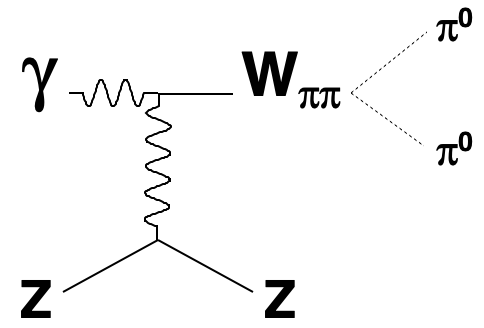
\includegraphics[height=3cm,clip=true]{figures/Diagram_Primakoff.png} \hspace{1cm}
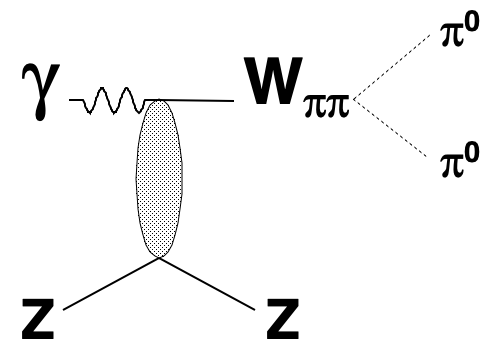
\includegraphics[height=3cm,clip=true]{figures/Diagram_hadronic.png}
\caption{Sketch of coherent two-pion production. Left) Signal: Primakoff mechanism, Right) Backgrounds: Other production mechanisms.
\label{fig:Diagram}}
\end{center}
\end{figure}

 \begin{figure}[tbh]
\begin{center}
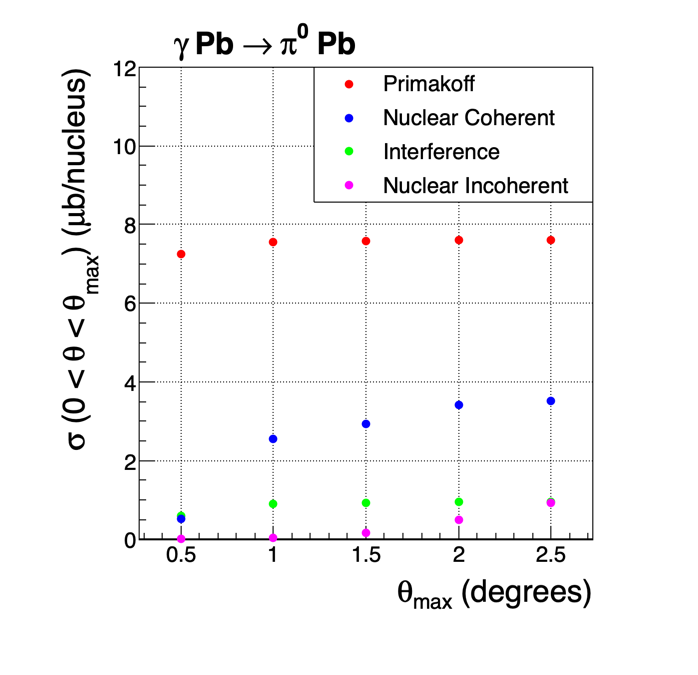
\includegraphics[height=5cm,clip=true]{figures/Primex_sigmas_c1.png} \hspace{1cm}
\caption{Integrated angular distribution for the $\pi^0$ in $\gamma\,Pb\rightarrow \pi^0\,Pb$ as a function of the upper limit of integration.
\label{fig:Primex_sigmas_c1}}
\end{center}
\end{figure}


We first classify the various backgrounds and then describe them in more detail one at a time. The exclusive production of two pions at threshold is very poorly known experimentally, and therefore there are large uncertainties in both the magnitude and the expected distributions of the backgrounds. We rely heavily on the measured single pion distributions, which are outlined in Fig.\,\ref{fig:Primex_sigmas_c1} and tabulated in Table\,\ref{tab:Primex_sigmas}. The major background comes from the $f0(500)$ $0^{+}$ meson that decays to two pions. The production mechanism is expected to very similar to single $\pi^0$ $0^{-}$ production, since the final states are the same except for parity. Therefore, we assume the relative background contributions to the single $\pi^0$ reaction will be similar in our experiment. Production inside the nucleus will tend to reduce hadronic backgrounds in the 2$\pi$ case due to absorption, but we take the conservative approach that absorption does not change the picture substantially. 

We have the following categories of backgrounds:
\begin{itemize}
\item Coherent production: In this case, the target remains intact. Generically, one may classify the two-pion production
according to the sketches in Fig.\,\ref{fig:Diagram}. The left-hand diagram represents the exchange of a virtual photon with the nucleus, i.e. the Primakoff
mechanism. This mechanism is very long range, approximately 100 fm, and is affected minimally by the effects of shadowing or absorption.  This is the signal for the
experiment and our goal is to determine its cross section.
The right-hand diagram represents the exchange of a strongly interacting particle (or trajectory) and effectively results in the production of pions at the
surface of the nucleus. We note that for the neutral pion production, pion exchange is not allowed due to charge conjugation conservation, while 
for the charged pion case, single pion exchange is related to the axial anomaly ($\gamma \pi^0 \rightarrow \pi^+ \pi^-$).  When the interaction leaves the
nuclear target intact, the reaction is referred to as ``nuclear coherent'' and this is our most serious background. 
\item Incoherent production:  When the interaction produces two pions in the quasi-elastic scattering off a single
nucleon, the scattered target usually fragments into particles that range out in the target and are unobservable experimentally. This reaction occurs at larger $-t$ and is generally
kinematically distinct from the signal. The $\pi^0\pi^0$ momentum relative to the photon polarization plane does differentiate between the Primakoff and incoherent production.
\item Any reaction that may be confused with the signal within the experimental resolution or limited acceptance:
 An example of this type of reaction is Primakoff production of $\eta$ mesons, where the $\eta\rightarrow \pi^0 \pi^0 \pi^0$  is
mis-reconstructed as a two-pion final state. 
\end{itemize}

We note that two important backgrounds for the charged-pion polarizability experiment do not contribute in this experiment:
First, coherent $\rho^0$ photo-production is absent in this
experiment because the $\rho^0$ decay into the $\pi^0\pi^0$ channel is prohibited by I-spin conservation.  Second, $\mu^+\mu^-$ production is also not a factor for the neutral pion case.

\subsection{Nuclear coherent background \label{sec:NCback}}
   
 The largest coherent background is  
from the $f_0(500)(J^{PC}=0^{++})$, also called the $\sigma$ meson, and the $f_0(980)$ photo-production.  The width of the
$f_0(980)$ is fairly narrow and does not contribute directly to the strength near threshold.
The $f_0(500)$ width is much
broader, from threshold to 800 MeV, with significant overlap in the
invariant mass region of interest.  Since the $f_0(500)$ is a scalar
particle with the same spin-parity as the $\gamma \gamma \rightarrow
\pi^0\pi^0$ final state near threshold, the azimuthal distribution of the $\pi^0\pi^0$ momentum relative to the
photon polarization plane does not differentiate between coherent
$f_0(500)$ production and the Primakoff reaction.  
This is similar to the Primex-$\pi^0$ experiment, where the dominant background was
nuclear coherent $\pi^0$ photo-production.  The approach used in the
Primex analysis was to measure the $\pi^0$ angular distribution,
effectively the $t$-distribution, then use theoretical calculations of
the angular distributions to separate out contributions from Primakoff
and nuclear coherent. The analysis of the $\pi^0\pi^0$ (NPP) reaction
will approximately parallel what was done for the Primex-$\pi^0$
analysis.  

We parameterize the $\sigma$ meson as detailed in Appendix\,\ref{sec:NCsigma} and assume that the production amplitude can be factorized as
\begin{eqnarray}
\mathcal{A} & = & \mathcal{A}_t(t) \, \mathcal{A}_W(m_{\pi\pi}) \, \mathcal{A}_\tau(\Phi, \phi, \theta),
\end{eqnarray}
where the last factor represents the angular distribution that results in a 
dependence on the di-pion azimuthal angle, $\phi_{\pi\pi}$, of the form $\mathcal{A}_\tau \propto (1 + \mathcal{P} \cos{2\phi_{\pi\pi}}$). 
The mass dependence is given by the S-wave phase shifts that dominate the mass region below 0.8 GeV. We use the approximate description given in 
Appendix\,\ref{sec:ParmSwave}.\footnote{More detailed studies may require including contributions from the D-wave and S-wave, I=2, amplitudes.} 

 \begin{figure}[tbh]
\begin{center}
%\includegraphics[height=5cm,viewport=250 180 0 360,clip=true]{CPP_production3}
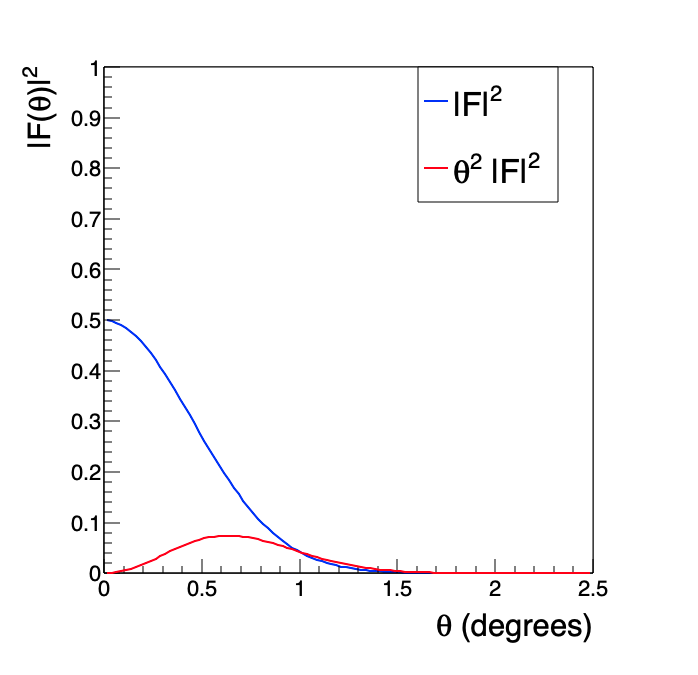
\includegraphics[height=5cm,clip=true]{figures/fit_Primakoff_sigma_c1.png}
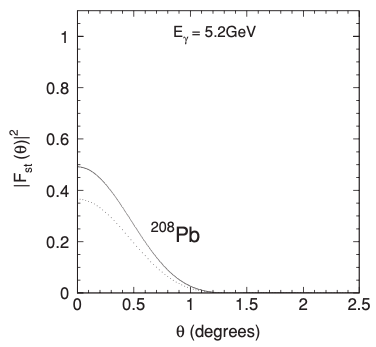
\includegraphics[height=5cm,clip=true]{figures/PRC80_2009_Fig6.png}
\caption{ Left) Approximation to strong form factor for lead, Right) Figure 6 from Ref.\,\cite{Gevorkyan:2009ge} showing the calculated strong form factor for single $\pi^0$ production off a lead target.
\label{fig:strongFF}}
\end{center}
\end{figure}

We assume the $-t$ dependence of the $\sigma$ has a similar form as for single $\pi^0$ production, namely $\mathcal{A}_t(t) \propto \sin{\theta_{\pi\pi}} \times F_{st}(t)$.  The $\sin{\theta_{\pi\pi}}$ 
comes from the spin-flip required at forward angles to produce a $0^+$ system from a spin-zero target. The factor $F_{st}(t)$ is the strong form factor for the target, which is approximated to
match calculations for the single $\pi^0$ production (Fig.\,6 from Ref.\cite{Gevorkyan:2009ge}). Our Gaussian approximation to the form factor is shown in Fig.\,\ref{fig:strongFF} along side the calculation for single 
$\pi^0$ production. Efforts are underway to calculate the strong form factor for this reaction.\footnote{S. Gevorkyan, private communication.}.
The Primex data showed that the nuclear coherent process is highly
suppressed for heavy nuclei, as shown in Fig.\ref{fig:leaddndt}.  The reason for the suppression is
$\pi^0$ absorption in the nuclear interior, making the coherent
production primarily a surface effect, i.e. proportional to $A$ and
not $A^2$.  For NPP it is expected that suppression of the nuclear  
coherent will be approximately twice stronger than that seen in Primex because two pions
are produced in NPP as compared to a single $\pi^0$ in Primex. 

 \begin{figure}[tbp]
\begin{center}
%\includegraphics[height=5cm,viewport=250 180 0 360,clip=true]{CPP_production3}
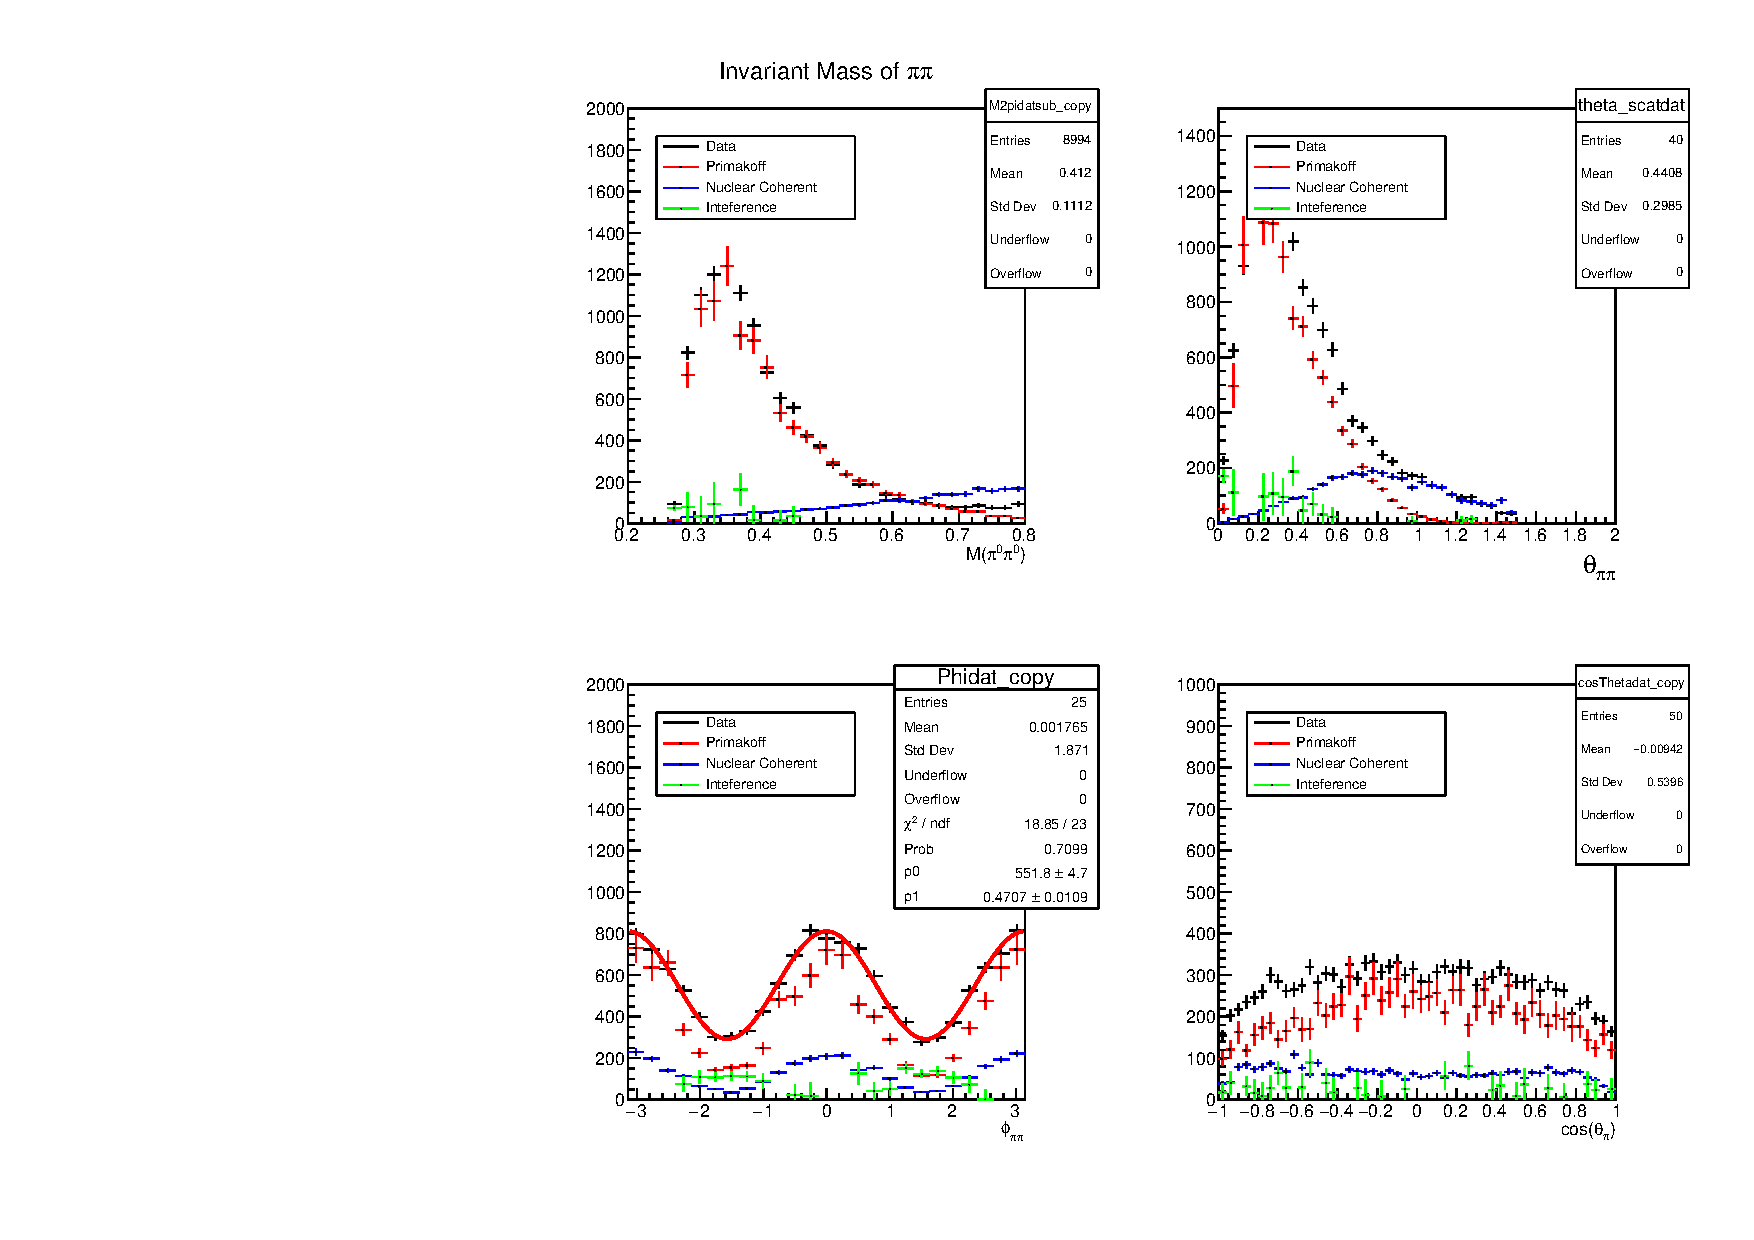
\includegraphics[height=15cm,clip=true]{figures/twopi_primakoff_DSelect_test_File_100000_decomposition_PrimNC.pdf}
\caption{Kinematic distributions for the Primakoff signal and nuclear coherent background.
Top left) Two-pi mass, Top right) Two-pi scattering angle, Bottom left) Two-pi azimuthal angle, 
Bottom right) Polar angle of one pion in the $2\pi$ center-of-mass.
\label{fig:decomposition_PrimNC}}
\end{center} 
\end{figure}


Figure\,\ref{fig:decomposition_PrimNC} shows distributions of interest for a sample of Primakoff signal and
nuclear coherent background events in an approximate proportion observed for single pion production. The strong phase between the two production mechanisms is set to
75 degrees for this simulation, where an angle of zero produces maximum interference. This angle must be determined experimentally. 
The distinguishing distributions are shown in the top panel: the 2$\pi$ mass and the 2$\pi$ scattering angle distributions. The Primakoff signal peaks at threshold and at about 0.2 degrees, whereas the nuclear coherent signal rises from threshold as expected from $f0(500)$ production and peaks at an angle of about 0.75 degrees. The azimuthal angular distribution is the same for both signal and background and has no discriminating power. The angular distributions of the pions in
the center of mass of the $2\pi$ system are all uniform, so do not help in distinguishing the signal from the nuclear coherent.  

\begin{figure}[tbp]
\begin{center}
%\includegraphics[height=5cm,viewport=250 180 0 360,clip=true]{CPP_production3}
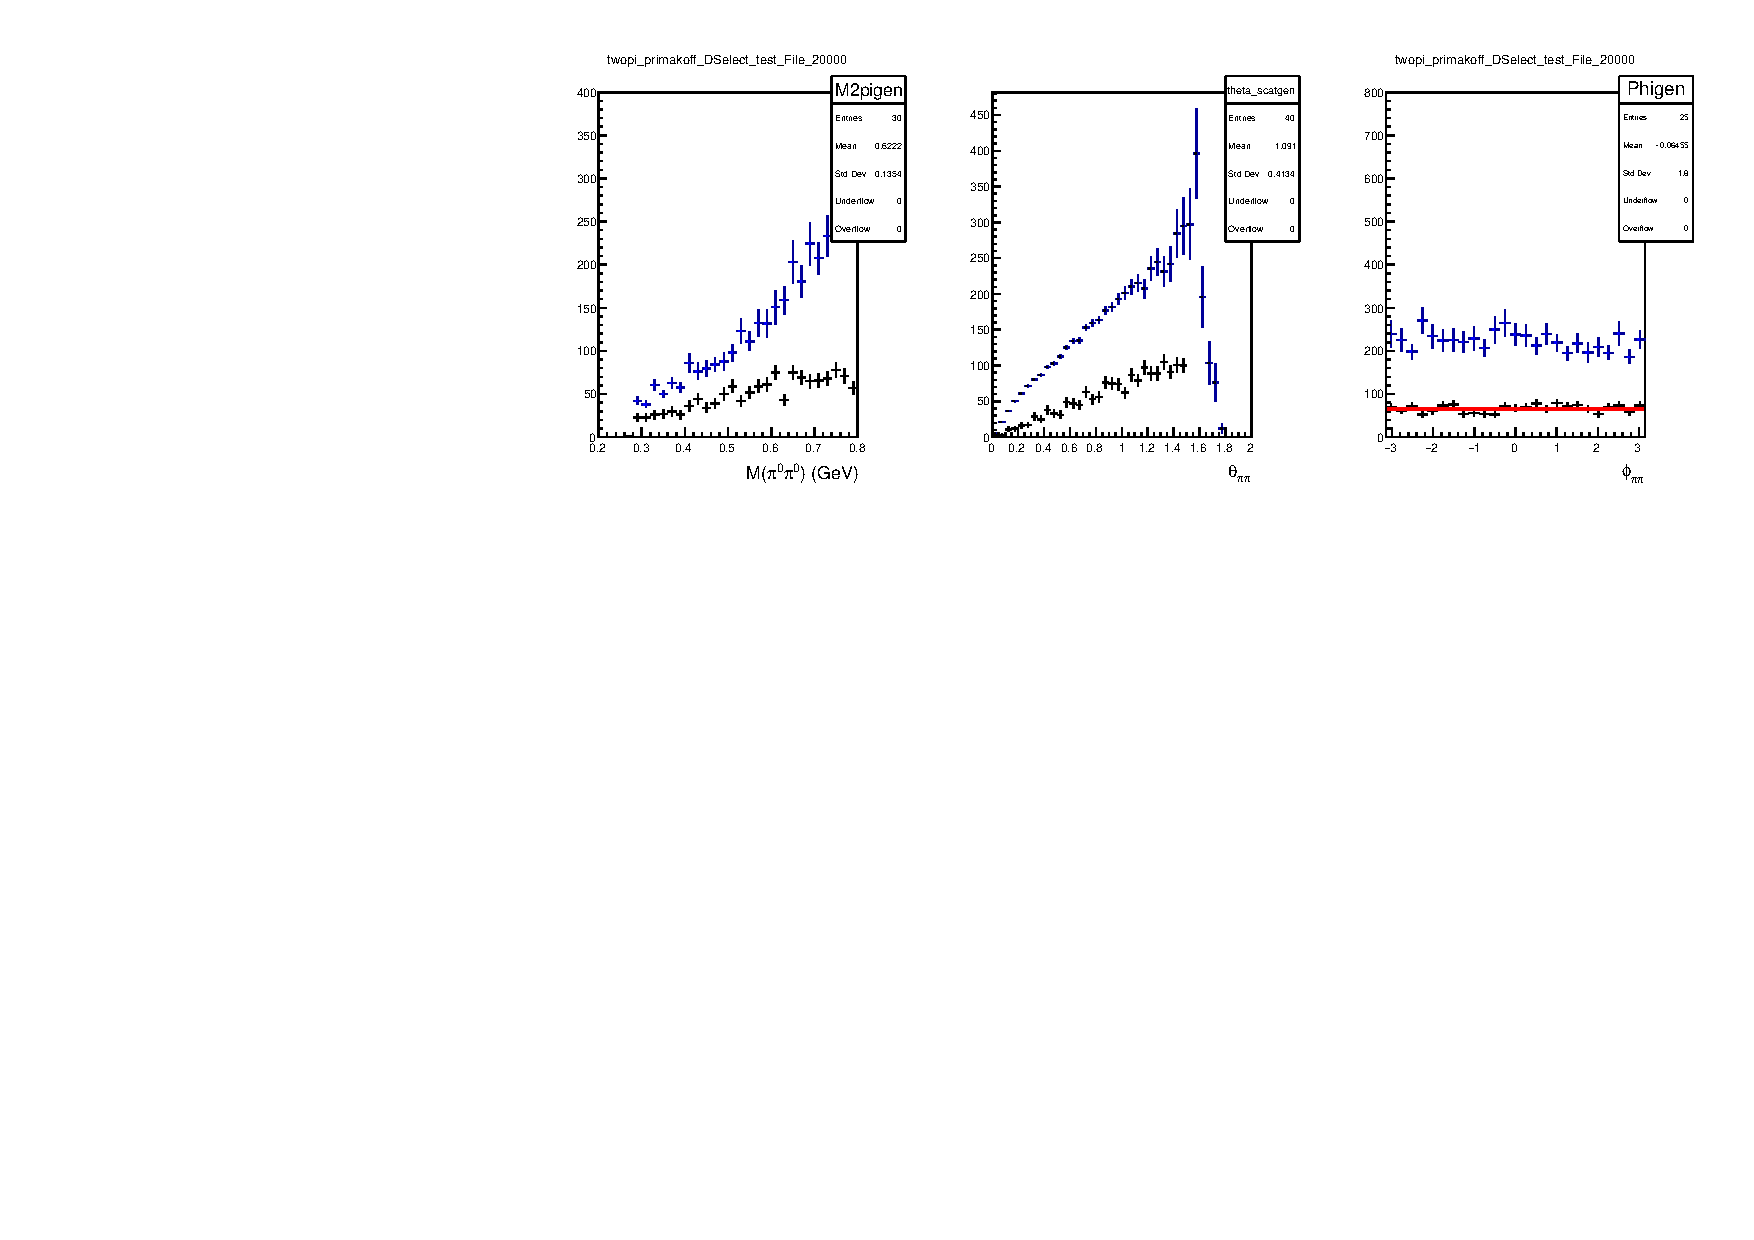
\includegraphics[width=16cm,clip=true]{figures/twopi_primakoff_DSelect_test_File_20000_IC.pdf}
\caption{Distributions for the incoherent production off free nucleons. The blue crosses represent the generated distributions and the black crosses represent the accepted and kinematically fit distributions.
Left) Two-pi mass. Center) Two-pi scattering angle. The drop of the generated distribution at 1.5 degrees is due to an analysis cut. Right) Two-pi azimuthal angle.
\label{fig:IC}}
\end{center} 
\end{figure}

\subsection{Incoherent two-pion production}
In addition to the coherent production of two pions off the nucleus, two pions may also be produced via the elementary reaction $\gamma N\to \pi^0 \pi^0 N$, breaking up the nucleus in the process. We model the incoherent background with a mass distribution given by the $f0(500)$, but with an exponential $t$ dependence given by $e^{Bt}$, with $B=3.6$ GeV$^{-2}$. The slope is taken from Ref.\cite{Battaglieri:2009aa} and has very large uncertainties. However, as long the slope is small compared to Primakoff production, which has an effective slope of $B\sim560$ GeV$^{-2}$, it does not change the picture. The mass and angular dependencies are shown in Fig.\,\ref{fig:IC}. The strength is small at threshold and at small angles, where Primakoff is strongest. The azimuthal angle is flat, so the photon polarization becomes an important tool in discriminating against this background. 

The cross section for this reaction on free protons is relatively large, about 140 nb/nucleon  for $0.3 < M_{\pi\pi} < 0.8$ GeV.\footnote{The cross section is estimated from the S-wave production of the $f0(500)$ meson extrapolated to small $-t$ from data archived in the {\em hepdata.net} database and reported in Ref.\,\cite{Battaglieri:2009aa}. See Appendix\,\ref{sec:NCsigma} for more information. A factor of one half is applied to the measured cross section for $\pi^+\pi^-$.} However, this process is strongly suppressed in nuclei by Pauli blocking and by pion absorption. The Pauli suppression is proportional to $1-G(t)$, where $G(t)$ is a nuclear form factor and has the limit of $G(t)\to1$ as $-t\to0$ \cite{Gevorkyan:2009ge,primex_inc}. In the case of single $\pi^0$ production, incoherent scattering contributes at the level of a couple of percent, and we expect it to be suppressed more strongly in $2\pi$ production. See Appendix\,\ref{sec:SigmaScaling} for details. Therefore, we expect this background to be about six times smaller than what is used in the present signal extraction studies.

\begin{figure}[tbp]
\begin{center}
%\includegraphics[height=5cm,viewport=250 180 0 360,clip=true]{CPP_production3}
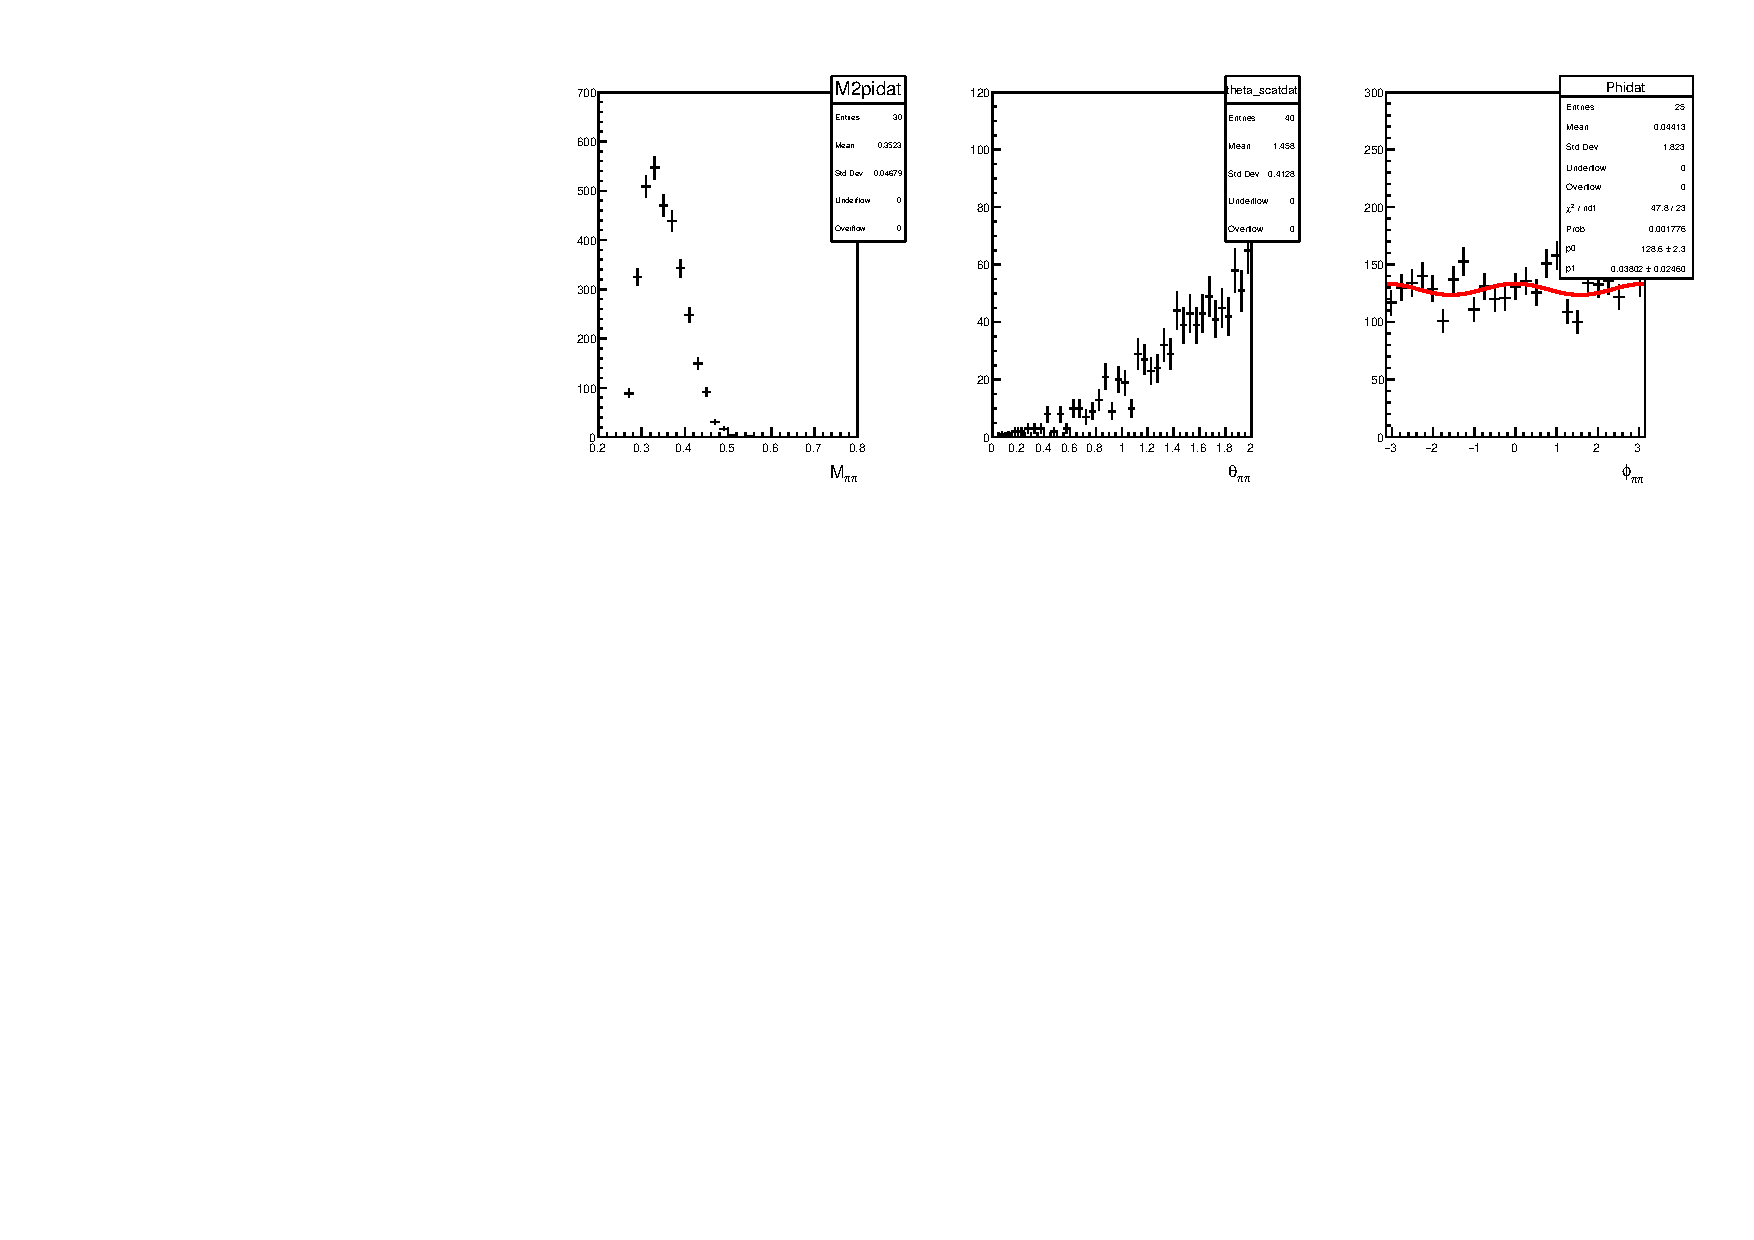
\includegraphics[width=16cm,clip=true]{figures/twopi_primakoff_DSelect_test_File_20000_eta.pdf}
\caption{Kinematically fit distributions for the $\eta$'s produced using the {\em genEtaRegge} event generator.
Left) Two-pi mass. Center) Two-pi scattering angle. Right) Two-pi azimuthal angle.
\label{fig:eta}}
\end{center} 
\end{figure}



\subsection{Miss-identified backgrounds}
There may be important backgrounds that are mistaken for the signal due to miss-identification. These may include
\begin{enumerate}[label=(\roman*)]
    \item coherent production of $\eta$ followed by $\eta\rightarrow \pi^0\pi^0\pi^0 \rightarrow \gamma\gamma\gamma\gamma(\gamma\gamma)$, where only four photons are reconstructed.
    \item production of nucleon resonances that contribute to the $\gamma N \rightarrow N \pi^0\pi^0$ final state. This contribution is expected to be small based on the experience of other Primakoff experiments.
\end{enumerate}
The first reaction is an inelastic, coherent process, and as such
could produce a significant rate for a heavy nuclear target. The kinematics of $\eta$ production was investigated using the {\em genEtaRegge} event generator \cite{hdnote2437}. This event generator has a fairly realistic description of $\eta$ production on hydrogen, including a contribution from the Primakoff reaction. However, it is missing the enhancement provided from scattering off a heavy target. The $\eta$'s were generated with the standard event-generator parameters and were decayed according to their nominal branching fractions. The events were then processed as for the Primakoff signal through the GEANT4 MC and {\em mcsmear}. These steps were followed through the event filter that analyzed the events assuming they were signal, i.e.  $\gamma Pb \rightarrow Pb\, \pi^0 \pi^0$ and a kinematic fit was performed assuming the target was missing. Standard missing-mass and $\chi^2$ cuts were used to pick out events that mimicked the signal. The distributions of the accepted events are shown in Fig.\ref{fig:eta}. 
We have scaled the event rate for $\eta$ production on lead using the scaling rules described in Appendix\,\ref{sec:SigmaScaling}, resulting in ten times the rate for Primakoff production of two pions ($\sim \Gamma_\eta\times Br(\eta \rightarrow \pi^0)/\Gamma_\sigma$).

We use a couple of very simple but powerful selection cuts to remove the $\eta$ background. The cuts include a selection on the missing mass squared ($|MM - M_{Pb}{^2}| < 0.1$ GeV$^2$) and a cut on the $\chi^2 < 5$ of the kinematic fit to $\gamma\,Pb\rightarrow \pi^0\pi^0 (Pb)$ with a missing recoil. In the analysis we also require a $2\pi$ scattering angle  ($\theta_{\pi\pi} <1.5$ degrees), which further restricts the range of missing mass. The result of these selections, which have been applied uniformly to signal and background, reduce the contamination from this source to about 16\% of the signal. These selections are illustrative and will allow us to achieve our experimental goals but further optimizations are likely. We note that the absolute number of mis-identified $\eta$'s in our signal region can be determined empirically from the measured rate of fully reconstructed $\eta\rightarrow\pi^0\pi^0\pi^0$ events.

 \begin{figure}[tbp]
\begin{center}
%\includegraphics[height=5cm,viewport=250 180 0 360,clip=true]{CPP_production3}
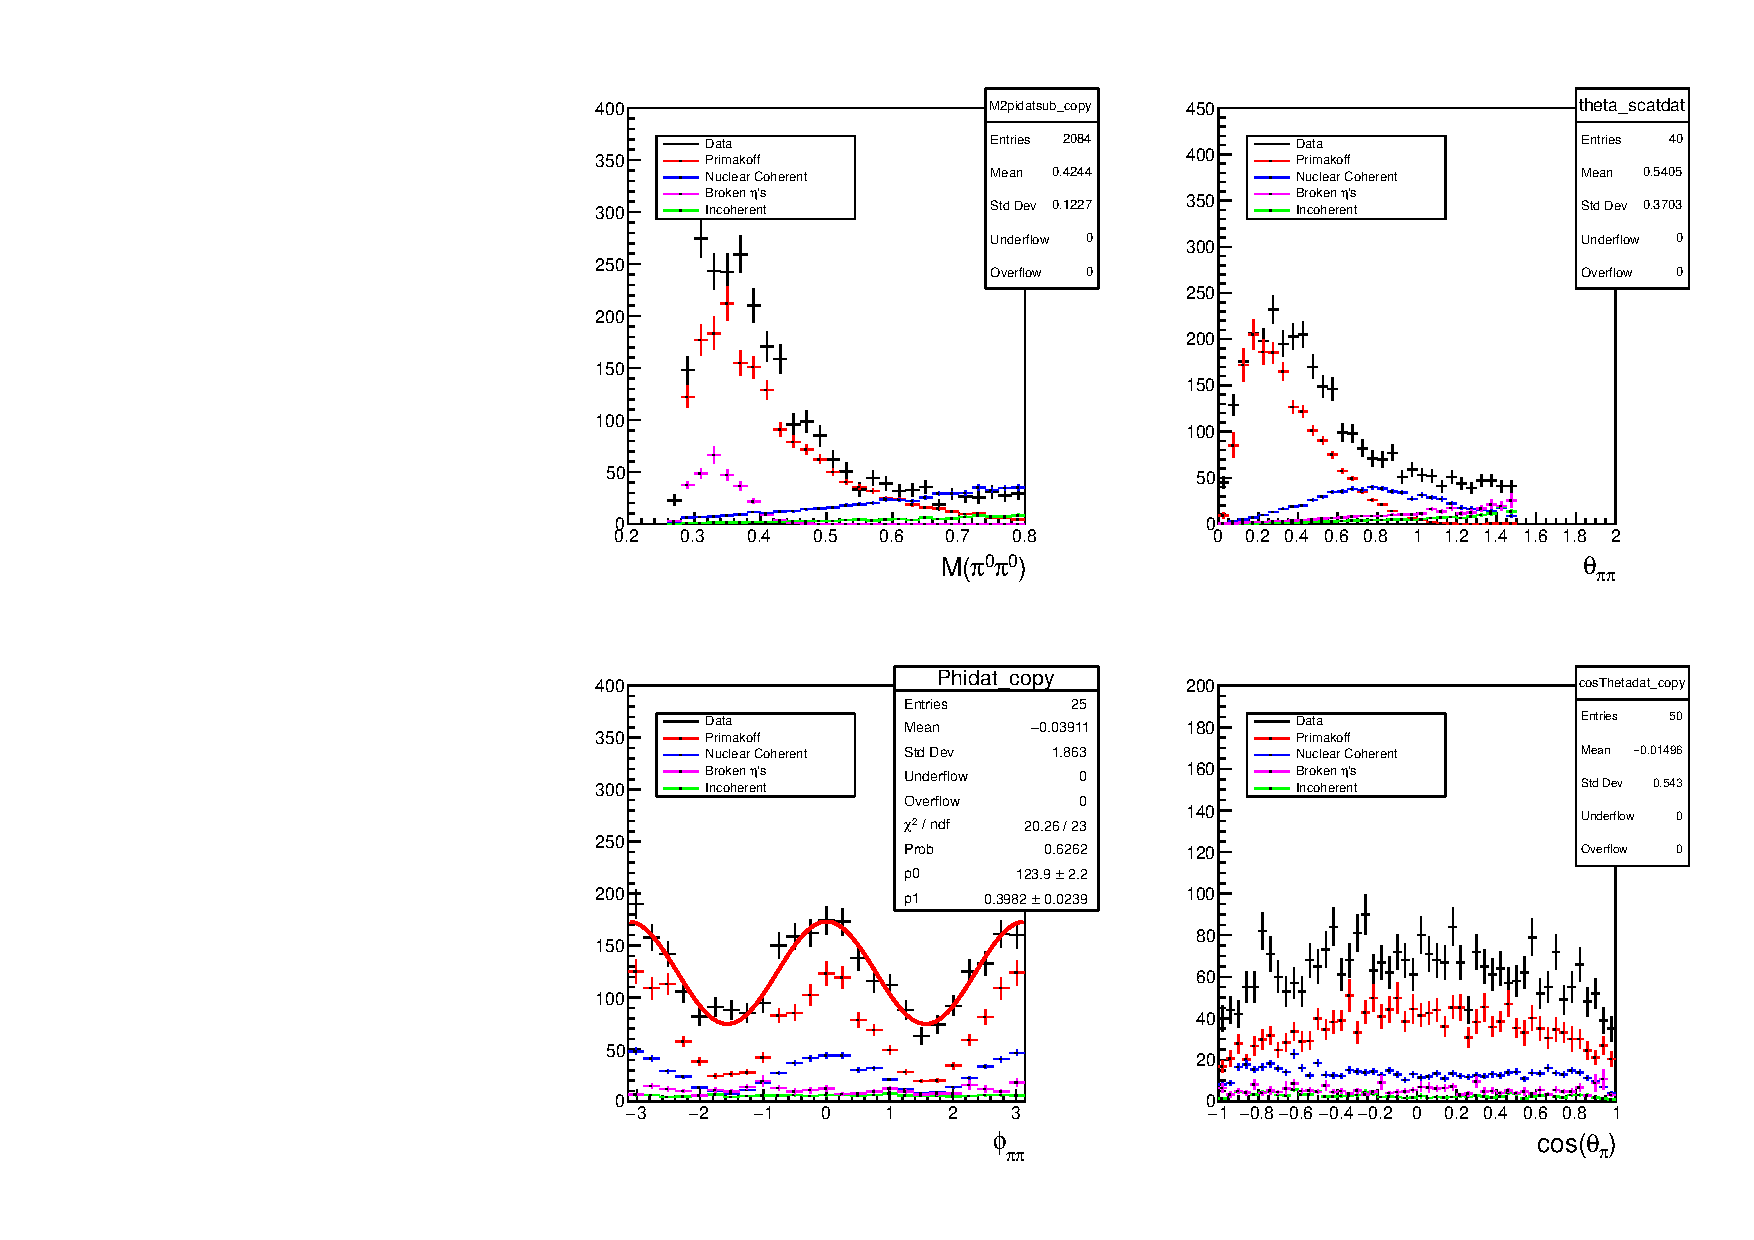
\includegraphics[height=15cm,clip=true]{figures/twopi_primakoff_DSelect_test_File_100000_decomposition_PrimNCICeta.pdf}
\caption{Kinematic distributions for the Primakoff signal and nuclear coherent background.
Top left) Two-pi mass, Top right) Two-pi scattering angle, Bottom left) Two-pi azimuthal angle, 
Bottom right) Polar angle of one pion in the $2\pi$ center-of-mass.
\label{fig:decomposition_PrimNCICeta}}
\end{center} 
\end{figure}

\subsection{Extraction of the Primakoff signal \label{sec:signalfit}}
The Primakoff signal is determined using an amplitude fit\footnote{AmpTools, https://github.com/mashephe/AmpTools/wiki.} to all data simultaneously. It assumes that the mass and angular distributions are know for each of the contributions to the 2$\pi$ sample. A complex scaling factor is determined for each contribution by doing an unbinned maximum likelihood fit to the event sample. The result of such a fit to the sample that includes the Primakoff and nuclear coherent processes only is shown in  Fig.\,\ref{fig:decomposition_PrimNC}. The fit to the data sample that also includes both incoherent and broken $\eta$'s is shown in Fig.\,\ref{fig:decomposition_PrimNCICeta}. The three kinematic quantities that are most discriminating between the signal and background are the 2$\pi$ mass $M_{\pi\pi}$, the 2$\pi$ scattering angle $\theta_{\pi\pi}$ and the azimuthal angle $\phi_{\pi\pi}$. The fit uses all the kinematic information contained in the event sample to determine the signal and background components that are present. As demonstrated in the figure, a good fit is obtained to the data and Primakoff signal is determined. The statistical uncertainties as a function of $M_{\pi\pi}$ are obtained directly from the fit (Top left plot in Fig.\,\ref{fig:decomposition_PrimNCICeta}). We estimate the systematic uncertainty (3\%) in the extraction of the signal by varying the fraction of incoherent in the sample. 

